\begin{figure}[ht]
	\centering
	\footnotesize

	\psfrag{an}[c][c] {$\text{\scriptsize Solid anode}$}
	\psfrag{ca}[c][c] {$\text{\scriptsize Solid cathode}$}
	\psfrag{fd}[c][c] {$\text{All-solid-state battery}$}
	\psfrag{ch}[c][c] {$\text{Sample: IEK - FZ Jülich}$}

	\psfrag{xx}[l][l] {$\text{Li}+$}
	\psfrag{xxx}[l][l] {$\text{Lithium Lanthanum Zirconate}$}
	\psfrag{em}[l][l] {$\text{e}-$}
	\psfrag{sele}[c][c] {$\text{\scriptsize Solid electrolyte}$}
	\psfrag{gr}[l][l] {$\text{Lithium metal}$}
	\psfrag{mo}[l][l] {$\text{Metal-oxide}$}
	\psfrag{xma}[l][l] {$\text{La}_{7}\text{Li}_{3}\text{Zr}_{2}\text{O}_{12}$}

	\psfrag{xbf}[l][l] {$\text{\scriptsize  No electric field}$}
	\psfrag{xat}[l][l] {$\text{\scriptsize  Under electric field}$}

	\psfrag{mic}[l][l] {$\text{Microscale: Part 2}$}
	\psfrag{mac}[l][l] {$\text{Macroscale: Part 1}$}
	\psfrag{sca}[c][c] {$\text{Scale}$}
	\psfrag{xgr}[c][c] {$\text{\scriptsize Grains}$}
	\psfrag{xgrb}[c][c] {$\text{\scriptsize Grain boundaries}$}
	\psfrag{gbb}[c][c] {$(\star)\ \text{\scriptsize Grain boundary}$}
	\psfrag{st}[l][l] {$(\star)$}
	\psfrag{g1}[c][c] {$\text{\scriptsize Grain 1}$}
	\psfrag{g2}[c][c] {$\text{\scriptsize Grain 2}$}

	\psfrag{xm}[c][c] {$-$}
	\psfrag{xp}[c][c] {$+$}
	\psfrag{dta}[c][c] {$\delta$}

	\psfrag{a}[c][c] {$\text{\faBolt}$}
	\psfrag{F}[c][c] {$\text{F}$}

	\psfrag{sse}[c][c] {$\text{Solid-state electrolyte}$}

	\psfrag{masca}[c][c] {$\text{Macroscale}$}
	\psfrag{mesca}[c][c] {$\text{Mesoscale}$}
	\psfrag{misca}[c][c] {$\text{Microscale}$}

	%--------------------------------------------------------

	\psfrag{seleb}[c][c] {$\text{\scriptsize Misorientation}$}
	\psfrag{selec}[c][c] {$\text{\scriptsize Multi-preferred directions}$}

	\psfrag{dispmu}[c][c] {$\text{Displacement field } \Bu$}
	\psfrag{pbar}[c][c] {$\Bu=\bar{\Bu}$}
	\psfrag{dbt}[c][c] {$\partial\Omega^{\Bt}_{N}$}
	\psfrag{dbphi}[c][c] {$\partial\Omega^{\Bu}_{D}$}
	%\psfrag{n}[c][c] {$\Bn$}
	\psfrag{n}[c][c] {$\Bn$}
	%\psfrag{tbar}[c][c] {$\Bt:=\Bsigma\cdot\Bn$}
	\psfrag{tbar}[c][c] {$\Bsigma\cdot\Bn = \bar{\Bt}$}
	\psfrag{phi}[c][c] {$\Bu$}


	\psfrag{concen}[c][c] {$\textsc{structure tensor } \BM^{R} \circ \BM^{E}$}
	%\psfrag{cbar}[c][c] {$c=\bar{c}$}
	\psfrag{cbar}[c][c] {$\phi=\bar{\phi}$}
	\psfrag{dbh}[c][c] {$\partial\Omega^{h}_{N}$}
	\psfrag{dbc}[c][c] {$\partial\Omega^{\phi}$}
	%\psfrag{n}[c][c] {$\Bn$}
	%\psfrag{hbar}[c][r] {$h := \KIh\cdot\Bn$}
	%\psfrag{hbar}[c][r] {$\KIH\cdot\Bn = \bar{H}$}

	\psfrag{c1}[c][c] {$\Bd^{R}_{G_1}$}
	\psfrag{c2}[c][c] {$\Bd^{R}_{G_2}$}

	\psfrag{gd1}[l][l] {$\text{Grain-1}$}
	\psfrag{gd1p}[l][l] {$\text{preferred}$}
	\psfrag{gd1d}[l][l] {$\text{direction}$}

	\psfrag{gd2}[c][c] {$\text{Grain-2}$}
	\psfrag{gd2p}[c][c] {$\text{preferred}$}
	\psfrag{gd2d}[c][c] {$\text{direction}$}

	\psfrag{ce}[c][c] {$\Bd^{E}$}

	\psfrag{rsbulk}[c][c] {$\text{rest of the bulk}$}
	\psfrag{mu}[c][c] {$\phi$}

	\psfrag{xb}[c][c] {$\Bx \in \Omega$}

	\psfrag{str}[c][c] {$\BM^{R} := \Bd^{R} \otimes \Bd^{R}$}
	\psfrag{mde}[c][c] {$\BM^{E} := \Bd^{E} \otimes \Bd^{E}$}

	\psfrag{cp}[c][c] {$\text{preferred direction}$}

	\psfrag{temp}[c][c] {$\text{Temperature field }  \theta$}
	\psfrag{te}[c][c] {$\theta$}
	\psfrag{tebar}[c][c] {$\theta = \bar{\theta}$}
	\psfrag{dbte}[c][c] {$\partial\Omega^{\theta}_{D}$}
	\psfrag{hbar}[c][c] {$\Bq\cdot\Bn = \bar{h}$}

	\psfrag{ecpu}[l][l] {$\text{Uniform}$}
	\psfrag{ecpep}[l][l] {$\text{electric-potential}$}
	% \psfrag{ecpid}[l][l] {$\text{induced direction}$}
	\psfrag{ecpid}[l][l] {$\text{polarizational effect}$}

	\psfrag{pl}[l][l] {$+$}
	\psfrag{mn}[l][l] {$-$}

	\psfrag{plc}[l][l] {$\textsc{Polycrystalline LLZO}$}

	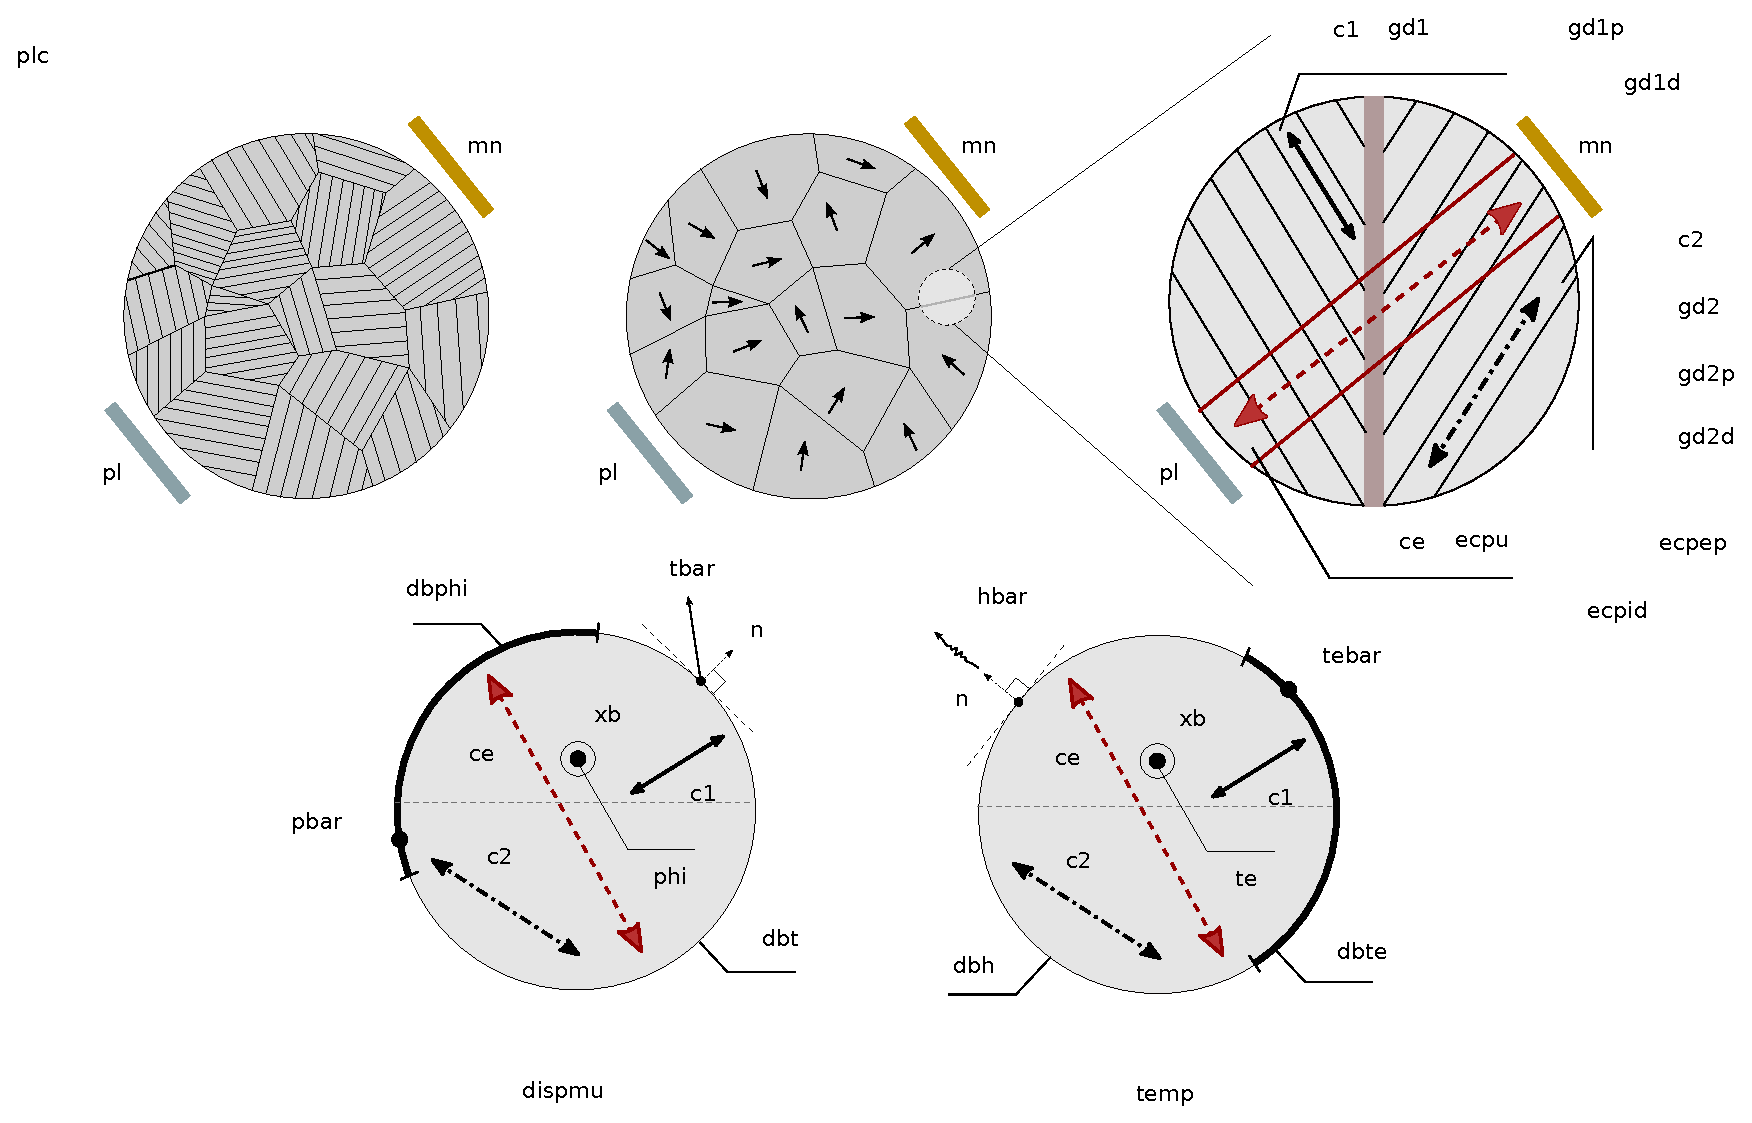
\includegraphics[width=0.8\textwidth]{multistructures.eps}
	\caption{Multi-structural internal variables $\Bd^{R}_{G_{i},i=1,\dots,N}$
	as referential material direction of $N^{th}$ grains, 
	and $\Bd^{E}$ as the globally uniform electric-potential direction,
	and the two governing fields in thermodynamically consistent continuum mechanics: 
	displacement $\Bu$ and temperature $\theta$.}
	\label{\LABEL}
\end{figure}
